\section{Hintergrund}
In diesem Kapitel wird auf die Konzepte und Begriffe von Webcrawlern und Machine Learning eingegangen. Es soll ein gemeinsames Grundwissen für beide Gebiete geschaffen werden.
%
\subsection{Webcrawler}
Um Informationen von Webseiten zu sammeln, muss deren Inhalt analysiert und die gewünschten Daten extrahiert werden. Für diese Aufgabe eignen sich Webcrawler besonders gut \cite{scrapy_1, scrapy_2}.\\
Dabei erhält ein Webcrawler eine oder mehrere Einstiegs-URLs. Diese werden dann vom Crawler aufgerufen und die dazugehörigen Seiten ausgewertet. Bei der Auswertung kann der Crawler auf weitere URLs stossen, die er in seine abzuarbeitende URL Liste aufnehmen kann. Sind alle URLs abgearbeitet ist der Crawler fertig. Je nach Aufgabenbereich existieren verschiedene Crawler-Techniken.\\
Ist bekannt von welchen Seiten die Informationen gecrawlt werden können, eignet sich am besten ein fokussierter Crawler. Dieser Crawler steuert vordefinierte Seiten an und extrahiert Informationen nach vorgegebenen Regeln.\\
Sind die Webseiten nicht bekannt oder kommt man nicht ohne weiteres an gesuchte Informationen, eignen sich Deep Web Crawler. Diese bewegen sich mehrheitlich autonom und versuchen durch Analysieren des Inhaltes herauszufinden ob der Inhalt von Interesse ist oder nicht.\\
Sind es übermässig viele Seiten, die gecrawlt werden müssen, oder ist die Stabilität der Crawler wichtig, kommen verteilte Crawler zum Einsatz. Durch die Verteilung wird an Stabilität gewonnen und die Last auf die verschiedenen Crawler verteilt \cite{scrapy_3}.\\[2ex]
%
Um Daten von einer Webseite zu extrahieren, gibt es diverse Möglichkeiten. Von der einfachen Stringsuche bis zu Machine Learning Methoden gibt es nahezu alles. Beim fokussierten Crawlen wird häufig versucht Informationen über den XPATH oder über die CSS-Klassen zu extrahieren. Beide Varianten haben ihre Vor- und Nachteile, sind aber im Grunde sehr ähnlich \cite{xpath_vs_css}. Somit ist es dem Benutzer überlassen welche Variante er wählt \cite{xpath}.\\[2ex]
%
Eine Herausforderung beim Crawlen ist, dass der Crawler nicht als solchen vom Webseitenbetreiber erkannt wird. Diverse Betreiber möchten gerne verhindern, dass Informationen von Ihren Seiten gecrawlt werden \cite{comparis}.\\
Ist ein Crawler zu aggressiv, kann es vorkommen, dass er vom Betreiber gesperrt wird. Es gilt daher mit einer gewissen Raffinesse vorzugehen. Um möglichst nicht aufzufallen, ist es sinnvoll nur ein paar Requests\footnote{Anfrage auf eine Webseite} pro Minute abzusetzen und einen existierenden User Agent anzugeben. Wenn das nicht ausreichend ist, können die Seiten über einen Pool von rotierenden IP-Adressen aufgerufen werden. So ist die Quelladresse nicht immer dieselbe \cite{offensive_crawling}.
%
\subsection{Machine Learning}
Machine Learning ist eine Art Künstliche Intelligenz (AI), das Softwareapplikationen erlaubt Vorhersagen zu machen, anhand von trainierten Algorithmen.
Die Definition von Machine Learning aus dem Jahr 1959 von Arthur Samuel, einer der Pioniere im Bereich Machine Learning, lautet \cite{what_is_ml}:
  \begin{quote}
    Machine Learning: Field of study that gives computers the ability to learn without being explicitly programmed.
  \end{quote}
Mit Hilfe von Machine Learning Algorithmen können neben Vorhersagen auch Trends erkannt oder Klassifizierungen durchgeführt werden \cite{ml_book}.
Dabei handelt es sich nicht um eine exakte Wissenschaft. Es lohnt sich verschiedene Algorithmen mit unterschiedlichen Parametern auszuprobieren, um die geeignetste Performance zu finden. Vieles hängt auch von den Ausgangsdaten ab \cite{ml_azure}.\\
%
Grundsätzlich erhält ein Algorithmus Daten, die er zu einem Modell verarbeitet. Dieses Modell wird ausgewertet. Entspricht es nicht den gewünschten Anforderungen wird versucht ein besseres Modell zu erstellen, bis das Resultat zufriedenstellend ist. Abbildung \ref{fig:ml_process} zeigt den schematischen Ablauf.\\
\begin{figure}[ht]
\centering
\begin{tikzpicture}[
  font=\sffamily,
  every matrix/.style={ampersand replacement=\&,column sep=1.5cm,row sep=.5cm},
  source/.style={draw,thick,rounded corners,fill=yellow!20,inner sep=.3cm},
  process2/.style={draw,thick,rounded corners,fill=blue!20,inner sep=.3cm},
  process/.style={draw,thick,circle,fill=orange!20},
  process3/.style={draw,thick,rounded corners,fill=orange!20, inner sep=.3cm},
  sink/.style={source,fill=green!20},
  datastore/.style={draw,very thick,shape=datastore,inner sep=.3cm},
  dots/.style={gray,scale=2},
  to/.style={->,>=stealth',shorten >=1pt,semithick,font=\sffamily\footnotesize},
  dotted/.style={dashed,->,>=stealth',shorten >=1pt,semithick,font=\sffamily\footnotesize},
  every node/.style={align=center}]
% Position the nodes using a matrix layout
\matrix{
  \node[source] (data) {Data};
      \& \node[process] (model) {Model};
        \& \node[sink] (prediction) {Prediction}; \\
};

% Draw the arrows between the nodes and label them.
\draw[to] (data) -- node[midway,above] {Train}
    node[midway,below] {} (model);

\draw[to] (model) -- node[midway,above] {Predict}
    node[midway,below] {} (prediction);

\draw[to] (prediction) to[bend right=50] node[midway,above] {Evaluate}
    node[midway,below] {} (data);
\end{tikzpicture}
\caption[Schematischer Ablauf bei Machine Learning]{Schematischer Ablauf bei Machine Learning}%
\label{fig:ml_process}
\end{figure}
\newline
%
Es gibt drei verschiedene Kategorien von Machine Learning \cite{super_unsuper}.\\
\textbf{Supervised Learning:}	Bei diesen Algorithmen sind die Daten gekennzeichnet. Das heisst, es ist erkenntlich, welchen Beobachtungswert die Daten darstellen. Mit Hilfe von diesen Daten, wird ein Modell erstellt, das möglichst nahe den Beobachtungswert schätzt. Dabei kann es sich um eine Klassifizierung oder Regression handeln.\\[2ex]
%
\textbf{Unsupervised Learning:} Hier hat man keine gekennzeichneten Daten. Es wird versucht Muster im Datensatz zu erkennen. Anhand von diesen können unter anderem Trends oder Ausreisser erkannt werden.\\[2ex]
%
\textbf{Reinforcement Learning:} Hier lernt der Algorithmus anhand seiner Aktionen. Für jede Aktion, die er berechnet, wird er entweder belohnt oder bestraft. Mit der Zeit kann der Algorithmus situationsbedingte Abläufe erlernen und später anwenden.\\[2ex]
%
Für eine Schätzung braucht jeder Machine Learning Algorithmus ein berechnetes Modell. Dieses kann unter anderem eine mathematische Formel oder eine Baumstruktur sein. Damit ein Modell erstellt werden kann, braucht jeder Algorithmus ein oder mehrere Features. Features sind messbare Merkmale, die einen Beobachtungswert, auch Target genannt, beschreiben. Es ist sinnvoll die Features im Voraus zu untersuchen und herauszufinden, welche Features wichtig sind und welche weggelassen werden können. Dabei können zwei oder mehrere Features kombiniert werden. Dieses Vorgehen wird auch Feature Engineering genannt.\\[2ex]
%
Damit ein Algorithmus überprüfen kann, wie gut seine Schätzungen sind, wird der Fehler, beziehungsweise die Residuals berechnet. Die Differenz zwischen einem geschätztem Wert und dem dazugehörigen beobachteten Wert wird als Residual bezeichnet. Dabei sind systematische\footnote{Ein falsches Modell wurde verwendet.} wie auch statistische Fehler\footnote{Es handelt sich um Ausreisser.} im Residual mit  eingerechnet. Formel \eqref{eq:residuals} zeigt die Berechnung des Residuals, dabei ist $\hat{y}$ der geschätzte Wert und y der beobachtete Wert. Es kann sich dabei sowohl um Skalare als auch Vektorenwerte handeln.\\
\begin{equation}
\label{eq:residuals}
\hat{\varepsilon} = y - \hat{y}
\end{equation}
%
\begin{table*}[hb]
\centering
\ra{1.3}
\resizebox{\textwidth}{!}{
\begin{tabular}{@{}llll@{}}
\toprule
Name & Abkürzung & Formel & Modelart\\
\midrule
Mean Absolute Error & MAE & $\frac1n \sum_{i=1}^{n} |y_i - \hat{y_i}|$ & absolut\\
Median Absolute Error & MdAE & $med(\sum_{i=1}^{n} |y_i - \hat{y_i}|)$ & absolut\\
Sum of Squared Errors & SSE & $\sum_{i=1}^{n} (y_i - \hat{y_i})^2$ & quadratisch\\
Root Mean Squared Errors & RMSE & $\sqrt{\frac1n \sum_{i=1}^{n} (y_i - \hat{y_i})^2}$ & quadratisch\\
Mean Absolute Percentage Error & MAPE & $\frac1n \sum_{i=1}^{n} |\frac{y_i - \hat{y_i}}{y_i}|, y_1 \neq 0$ & prozentual\\
Median Absolute Percentage Error & MdAPE & $med(\sum_{i=1}^{n} |\frac{y_i - \hat{y_i}}{y_i}|), y_1 \neq 0$ & prozentual\\
\bottomrule
\end{tabular}}
\caption{Fehlermodelle mit Formelen}
\label{tab:error_models}
\end{table*}
%
Wie in Tabelle \ref{tab:error_models} gezeigt, haben sich mit der Zeit diverse Fehlermodelle entwickelt. Die Wahl des Fehlermodells ist vom Anwendungsfall abhängig. Grundsätzlich können Fehler absolut oder quadratisch berechnet werden \cite{error_models}.\\
Bei absoluten Werten werden alle Fehler gleich stark gewichtet, wobei bei quadratischen Fehler grössere Fehler durch das Quadrieren stärker gewichtet werden. Beim MAE hat ein Fehler bei einem hohen Beobachtungswert einen grösseren Einfluss auf den gesamten Fehler. Das kann durch den Median (MdAE) oder einer prozentualen Angabe wie der MAPE oder MdAPE vermieden werden. Eine prozentuale Angabe hat zusätzlich den Vorteil, dass sie intuitiver Interpretiert werden kann. Der Nachteil bei MAPE und MdAPE ist, dass sie bei einem y Wert von 0 nicht verwendet werden können \cite{error_models_2}.\\[2ex]
%
Eine weitere Möglichkeit die Performance eines Modells neben dem Fehlermodell zu bestimmen, ist der $R^2$ Wert. $R^2$ ist ein Gütemass, das beschreibt, wie gut die Features in der Lage sind, die Varianz der Zielvariable erklären zu können. Die Formel \eqref{eq:r2} zeigt, dass der Wert immer zwischen 0 bis 1 liegt. Dabei ist y der Beobachtungswert, $\hat{y}$ der geschätzte Wert und $\overline{y}$ der Durchschnitt aller y. Sind alle Beobachtungswerte gleich ist $R^2$ nicht definiert. Je näher sicher der Wert bei 1 befindet, desto besser ist das Modell.\\
Es gilt jedoch zu beachten, dass der $R^2$ Wert die Varianzen aufzeigt. Somit kann nicht davon ausgegangen werden, dass ein hoher $R^2$ Wert auch eine hohe Genauigkeit beim Schätzen erzielt \cite{r2, r2_2}.
\begin{equation}
\label{eq:r2}
R^2 = 1 - \frac{\sum_{i=1}^{n} (y_i - \hat{y_i})^2}{\sum_{i=1}^{n}(y_i - \overline{y})^2},\text{ falls nicht }y_1  = ... = y_n = \overline{y}
\end{equation}
%
Es macht keinen Sinn auf denselben Daten zu trainieren und das Modell zu überprüfen. Deshalb wird der Datensatz in mindestens einen Trainings- und einen Testdatensatz aufgeteilt \cite{cross_validation}.
Dadurch kann die Gefahr eines Overfit verringert werden. Bei einem Overfit wurde das Modell zu stark an den Testdaten trainiert. Wichtig dabei ist, dass die Daten vor dem Aufteilen gründlich gemischt werden. So, dass nicht alle Wohnungen im Trainingsdatensatz sind und nicht alle Häuser im Testdatensatz.\\
Cross Validation ist eine weitere Möglichkeit den Datensatz aufzuteilen. Dieser teilt den gesamten Datensatz in K-Teile auf. Dabei werden K-1 Datensätze für das Trainieren und 1 Datensatz für das Testen verwendet. Das ganze wird K-mal wiederholt, so, dass jeder Datensatz einmal als Testdatensatz verwendet wurde.
%
\subsubsection{Lineare Regression}
Bei der Linearen Regression versucht man anhand einer linearen Funktion einen Beobachtungswert y durch einen oder mehrere Features X zu berechnen. Dabei handelt es sich um ein statistisches Verfahren bei dem davon ausgegangen wird, dass y abhängig von X ist. Weiter gilt, dass die unabhängigen Variablen X dichotom oder intervallskaliert sind.
\begin{equation}
\label{eq:linear}
\hat{y} = h_\theta(x) = \sum_{j=0}^{N} \theta_j x_j
\end{equation}
Formel \eqref{eq:linear} zeigt die Lineare Regression wobei  den Koeffizienten für jedes einzelne Feature darstellt. Je höher der Koeffizient ist, desto mehr Gewicht hat dieses Feature im Modell. Um auf die optimalen Koeffizienten zu kommen, versucht der Algorithmus eine Gerade durch den Datensatz zu ziehen, die den kleinsten Abstand zu allen Punkten hat. Sprich, der Algorithmus versucht das Schätzungsmodell auf das gewählte Fehlermodell zu optimieren. Zugleich dient das Fehlermodell auch als Performancemetrik. Die Optimierung wird durch die Kostenfunktion \eqref{eq:cost_function} berechnet. Oft wird dafür die \textit{Ordinary least squares} (OLS) Methode genommen. Es gibt auch noch weitere Methoden für die Optimierung.\\
Das quadratische Fehlermodell macht den Algorithmus anfälliger auf Ausreisser. Diese sollten, wenn immer möglich, in einem vorherigen Schritt ausgemustert werden. Auch sollte der Fehler in den Daten normalverteilt sein und die Residuen eine Homoskedastizität aufweisen, da ansonsten keine gute Regression gefunden wird \cite{gradient_descent, gradient_descent_2, gradient_descent_3}.
\begin{equation}
\label{eq:cost_function}
J(\theta) = \frac{1}{2m} \sum_{i=1}^{N} (h_\theta(x^i) - y^i)^2
\end{equation}
%
\textbf{Polynomial Regression}\\
In vielen Fällen hat der Datensatz keine Homoskedastizität, sondern besitzt eine Heteroskedastizität \cite{poly}. Dies ist oft dann der Fall wenn das Verhältnis zwischen y und X einer Kurve entspricht. In solch einem Fall, erzielt die Lineare Regression keine gute Performance.
Bei der Polynomialen Regression ist deshalb der beste Fit keine Gerade, sondern ähnelt einer Kurve. Je nachdem wie viele Polynome die Funktion besitzt, desto kurvenreicher ist die Funktion am Schluss.\\
Die Formel für eine Polynom Gleichung zweiten Grades wird in Gleichung \eqref{eq:poly} dargestellt.
%
\begin{equation}
\label{eq:poly}
y = \theta_1 + \theta_2 * X + \theta_3 * X^2
\end{equation}
%
\newline
Je höher der Grad des Polynoms, desto genauer wird der Algorithmus auf den Trainingsdatensatz trainiert. Das hat den Nachteil, dass neue Datensätze ungenau geschätzt werden, da das Modell eine hohe Varianz aufweist. Dieses Phänomen nennt sich Overfitting. Der Algorithmus wurde zu stark am Trainingsdatensatz trainiert.\\
Ist der Grad des Polynoms zu klein gewählt, kommt es zu einem Underfitting. Das Modell kann nur Features abbilden, die dem ausgewählten Grad entsprechen. Alle anderen Features werden ignoriert. So entsteht die Gefahr, dass wichtige Features nicht ins Modell miteinfliessen und das Modell einen hohen Bias besitzt. Abbildung \ref{fig:under_overfit} zeigt den Vergleich von Underfit zu einem Overfit.\\
Es wird auch von dem \textit{Bias-Varianz-Dilemma} gesprochen \cite{bias_variance, bias_variance_2}. Denn die Kunst ist, die richtige Abstimmung zu finden, damit das Modell die beste Performance hat.
\begin{figure}[ht]
\centering
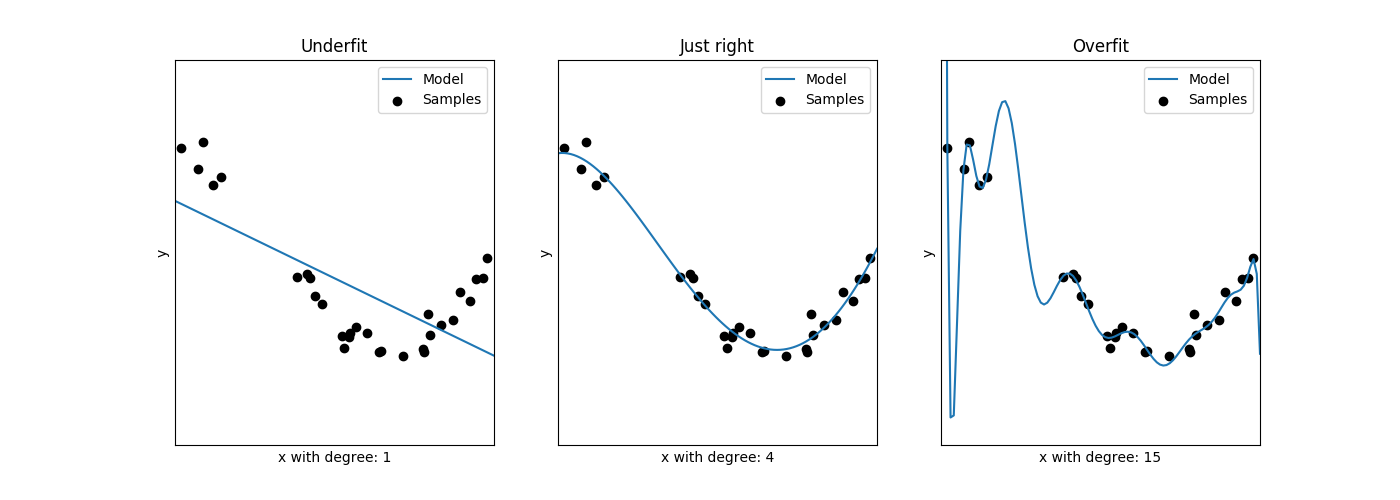
\includegraphics[width=\textwidth]{images/overfit_underfit.png}
\caption[Vergleich von Overfit zu Underfit]{Vergleich von Overfit zu Underfit}%
\label{fig:under_overfit}
\end{figure}
%
Das Bias-Varianz-Dilemma ergibt sich durch die Komplexität eines Modells. Die Komplexität wird durch das Hinzufügen von Polynomen oder Features gesteigert.
Es ist daher sinnvoll die Modelle möglichst einfach zu gestalten oder einen Regularisierungsparameter zu verwenden.\\[2ex]
%
\textbf{Ridge Regression}\\
Der Ridge Regression ist ein Linearer Regressions Algorithmus mit einem Regularisierungsparameter $\lambda$. Anhand diesem kann er die Koeffizienten der einzelnen Features verkleinern und somit die Komplexität reduzieren. Infolgedessen wird bei diesem Algorithmus auch Schrumpfparameter genannt. Je höher dieser gewählt wird, desto schwächer werden die Koeffizienten und somit das Modell einfacher \cite{ridge, ridge_2}. Formel \eqref{eq:ridge} zeigt die Definition des Ridge Algorithmus.
%
\begin{equation}
\label{eq:ridge}
J(\theta) = \frac{1}{2m} \sum_{i=1}^{N} (h_\theta(x^i) - y^i)^2 + \lambda \sum_{j=0}^{M} \theta_{j}^{2}
\end{equation}
%
\newline
Wichtig beim Ridge Algorithmus ist, dass die einzelnen Koeffizienten verkleinert werden, aber nie 0 erreichen. Das geeignetste Lambda hängt immer vom Datensatz ab und muss durch Analysieren verschiedener Werte gefunden werden.\\[2ex]
%
\textbf{Lasso Regression}\\
Ein weiterer Regularisierungs Algorithmus ist der Lasso Regression Algorithmus \eqref{eq:lasso}. Dieser fügt, wie der Ridge Regression auch, einen zusätzlichen $\lambda$ Parameter ein. Er nimmt dabei nicht das Theta im Quadrat, sondern den absoluten Wert von Theta und summiert diesen auf. Durch das kann der Algorithmus unwichtige Features auf 0 setzen und somit eliminieren. Wenn Features weggelassen werden, wird die Komplexität des Modells reduziert \cite{lasso}.
%
\begin{equation}
\label{eq:lasso}
J(\theta) = \frac{1}{2m} \sum_{i=1}^{N} (h_\theta(x^i) - y^i)^2 + \lambda \sum_{j=0}^{M} |\theta_j|
\end{equation}
%
%
\subsubsection{K-Nearest Neighbour}
Der K Nearest Neighbour Algorithmus (KNN) ist ein unsupervised Algorithmus und kann für Klassifizierungs- wie auch für Regressionsmodelle verwendet werden. In dieser Arbeit wird er als Regressionsmodell verwendet.\\
Der KNN-Algorithmus sucht für einen Punkt die K-nächsten Punkte, die er aus dem Trainingsset kennt. Als Schätzung gibt er den Durchschnitt der gefundenen Werten ab \cite{knn_1}.
KNN ist definiert als
\begin{equation}
\label{eq:lasso}
\hat{y} = \frac{1}{K} \sum_{i=1}^{K} (y_{knj})
\end{equation}
%
Wobei $\hat{y}$ der geschätzte Wert darstellt, $K$ die Anzahl Elemente, die für die Schätzung einbezogen werden und $y_{knj}$ die gefundenen beobachtungs Werte, die am nächsten zum gesuchten Punkt liegen.\\
Die Distanzberechnung von einem gesuchten Punkt kann mit unterschiedlichen Algorithmen berechnet werden. Häufig wird der Euklid, wie in Formel \eqref{eq:euklid} gezeigt, verwendet, da er alle Dimensionen gleich behandelt. Wie beim quadratischen Fehlermodell, ist auch der Euklid anfällig auf grosse Ausreisser. Um das zu verhindern, kann der Manhatten oder Chebyshev Algorithmus verwendet werden. Beim Manhatten Algorithmus werden Queerdistanzen höher gewichtet als gerade Distanzen. Im Gegensatz zum Chebyshev Algorithmus, bei dem alle Richtungen gleich gewichtet werden.
\begin{equation}
\label{eq:euklid}
D(x, p_i) = \sqrt{(x - p_i)^2}
\end{equation}
%
\newline
Auch bei diesem Algorithmus gibt es die Gefahr von einem Underfit beziehungsweise Overfit. Wählt man K zu gross, kommt es zu einem Underfit. Ist K sehr klein kann es zu einem Overfit kommen. Das Optimale K hängt vom Datensatz und der gewünschten Performance ab. Abbiludng \ref{fig:under_overfit_knn} zeigt den Vergleich von einem Underfit zu einem Overfit bei einem KNN Algorithmus.\\[2ex]
\begin{figure}[ht]
\centering
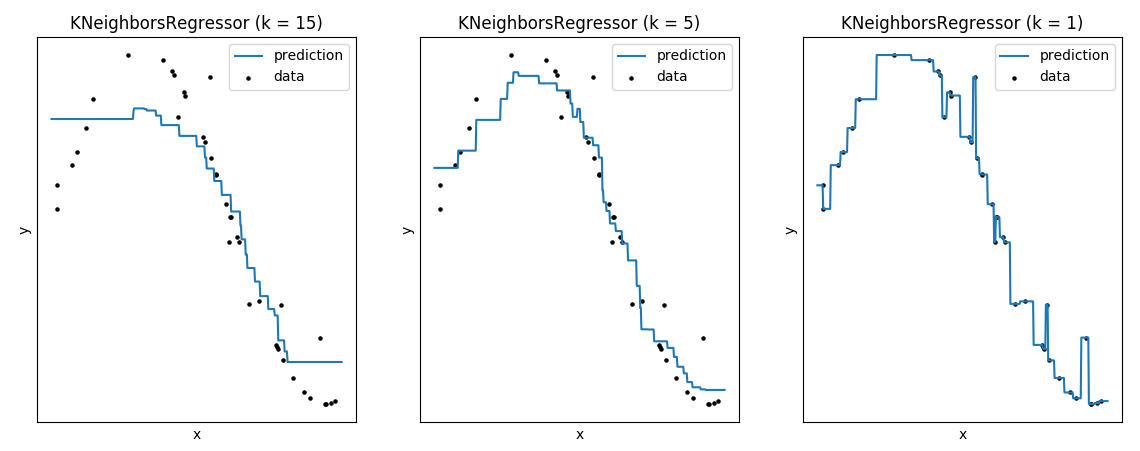
\includegraphics[width=\textwidth]{images/knears_overfit.png}
\caption[Vergleich von Overfit zu Underfit bei einem KNN]{Vergleich von Overfit zu Underfit bei einem KNN}%
\label{fig:under_overfit_knn}
\end{figure}
%
Der KNN Algorithmus kann erweitert werden, indem näher gelegene Punkte stärker gewichtet werden als weiter entfernte. So ist der Algorithmus weniger anfällig auf unregelmässige Daten oder Ausreisser.\\
Für die Gewichtung eines Punktes wird folgende Formel verwendet \eqref{eq:knn_weights}:
\begin{equation}
\label{eq:knn_weights}
W(x, p_i) = \frac{e^{(-D(x, p_i))}}{\sum_{i=1}^{K} e(-D(x, p_i))}
\end{equation}
%
$D(x, p_i)$ ist die Distanz vom gesuchten Punkt x zum nächsten Punkt i im Trainingsset. Da immer durch die Summe aller Distanzen dividiert wird, ist der Wert zwischen 0 und 1. Näher gelegene Punkte erhalten somit eine höhere Gewichtung W. Die Summe aller Gewichte ergibt immer 1.\\
Die Gewichtung wird dann mit dem gefundenen Beobachtungswert multipliziert, wie in Formel \eqref{eq:knn_with_weights} gezeigt. Die Durchschnittsberechnung muss nicht durchgeführt werden, da die Gewichtung normalisierte Werte zurückgibt \cite{knn_2, knn_3}.
\begin{equation}
\label{eq:knn_with_weights}
\hat{y} = \sum_{j=1}^{K} W(x_0, x_i) y_i
\end{equation}
%
%
\subsubsection{Tree Based Learning Algorithmen}
Ein anderer Ansatz von Machine Learning besteht aus den Tree Based Learning Algorithmen. Am verbreitetsten sind Classification and Regression Trees (CART), die von Breiman 1984 beschrieben wurden. Darunter gibt es noch diverse andere Algorithmen\footnote{ID3, C4.5, CHADI, MARS, Conditional Inference Trees}. Bei diesen Algorithmen handelt es sich grundsätzlich um supervised Algorithmen. Es existieren aber auch unsupervised Ansätze, die nicht Teil von dieser Arbeit sind.\\[2ex]

\textbf{Decision Trees}\\
\begin{figure}[ht]
  \centering
  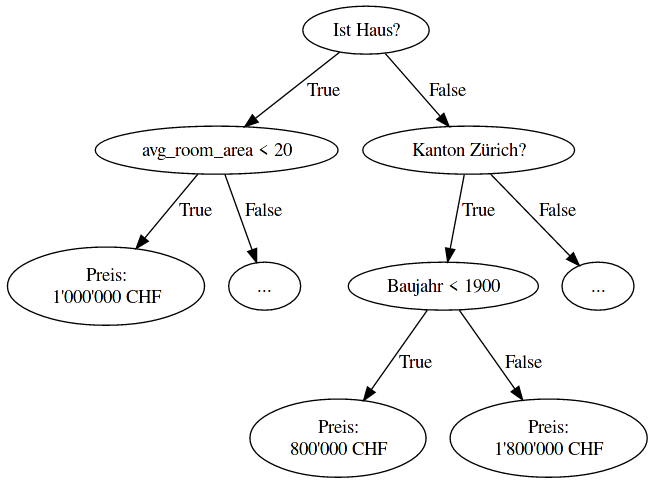
\includegraphics[width=\textwidth]{images/decision_tree.png}
  \caption[Decision Tree]{Decision Tree}%
  \label{fig:decision_tree}
\end{figure}
Ein Decision Tree (Entscheidungsbaum) ist eine Baumstruktur, die es erlaubt, Daten mithilfe von Entscheidungsregeln zu kategorisieren. Bei den Daten kann es sich sowohl um diskrete als auch um kontinuierliche Werte handeln.\\
Auf jedem Knoten des Entscheidungsbaumes wird ein Feature aus dem Datensatz ausgewählt und eine Teilung in seinem Wertebereich durchgeführt. Der Feature Raum wird somit in unterschiedliche, nicht überlappende Regionen aufgeteilt.\\[2ex]
Es gilt zu beachten, dass dasselbe Feature wiederholt als Entscheidungsregel verwendet werden kann.\\
Für eine Schätzung wird dann der Durchschnitt aller Werte in der Regionen $R_j$ berechnet, in die der zu schätzende Wert fällt.\\
Wie die  J unterschiedliche Regionen aufgeteilt werden, hängt von der Kostenfunktion ab. Bei der Regression wird dafür den Residual Sum of Squares (RSS) verwendet. Das Ziel ist es die Regionen $R_1$, $R_2$ … $R_j$ so zu legen, dass der RSS minimiert wird. Das kann anhand der Formel \eqref{eq:decision_tree} erreicht werden.
\begin{equation}
\label{eq:decision_tree}
\sum_{j=1}^{J} \sum_{j \in R_j}^{} (y_i - \hat{y}_{R_j})^2
\end{equation}
%
\newline
Dabei ist $\hat{y}_{R_j}$ jder durchschnittliche Beobachtungswert in der j-ten Region.
Für eine Klassifikation gibt es andere Kostenfunktionen wie der Gini Coefficent oder der Gini Impurity.\\
Da es aber mit steigender Anzahl von Datensätzen praktisch unmöglich wird, jede mögliche optimale Region durchzurechnen, wird ein “greedy” Ansatz verwendet. Greedy deshalb, weil die nächstbeste Teilung nur mit den aktuell vorhandenen Regionen berechnet wird. Es wird nicht rekursiv vorausberechnet um mit weiteren Teilungen ein theoretisch besseren Baum zu erstellen. So wird nur ein lokales und kein globales Optimum gefunden. Die Aufteilung einer Region in zwei unterschiedliche Regionen nennt sich “recursive binary splitting” und wird in Formel \eqref{eq:splitting} gezeigt. Dabei gilt die Bedingung für die zuteilende Region R wenn s die Entscheidungsregel ist.
%
\begin{equation}
\label{eq:splitting}
R_1(j,s) = \{X|X_j < s\} \text{and} R_2(j,s) = \{X|X_j \geq s\}
\end{equation}
%
\newline
Diese Splits werden solange rekursiv ausgeführt, bis eine der folgenden Abbruchbedingung erfüllt ist:
\begin{itemize}
\item Die minimale Anzahl an Datensätzen in einer Region ist erreicht.
\item Die maximale Tiefe wurde für einen Teilbaum erreicht.
\item Ein erneuter Split bringt keine besseren Ergebnisse.
\end{itemize}
Die Vorteile vom Decision Tree bestehen darin, dass der generierte Baum einfach, verständlich und lesbar ist, da das Endresultat ein geordneter und gerichteter Baum ist. Dadurch lässt sich dieser bei Bedarf auch gut visualisieren und Predictions können manuell überprüft werden, sofern der Baum nicht zu gross ist.\\
Decision Trees neigen jedoch gerne zu Overfitting. Dagegen hilft einerseits Pruning, andererseits Ensemblemethoden.\\
Pruning eliminiert bestehende Knoten, die sich als irrelevant herausstellen, anhand einem regularisierungs Parameter $\lambda$. Dieses Parameter ist ähnlich wie beim Lasso Algorithmus. Pruning ist jedoch nicht so verbreitet wie die Ensamblemethoden.\\[2ex]
%
\textbf{Random Forest}\\
Der Random Forest gehört in die Kategorie der Ensemblemethoden. Es handelt sich hierbei um einen erweiterten Bootstrap Aggregating (Bagging) Algorithmus und wurde von Breiman entwickelt. Bagging reduziert die Varianz indem der Algorithmus mehrere Bäume aus dem Datensatz generiert und diese einzeln trainiert.  Die Bäume bestehen jeweils aus einer zufälligen Teilmenge des ganzen Datensatz. Für die Schätzung wird dann der Durchschnitt aller Bäume B verwendet wie in Formel \eqref{eq:random_forest} gezeigt. Dabei ist $f^{(b)}$ die Schätzung für den b-ten Baum.
%
\begin{equation}
\label{eq:random_forest}
\hat{f_{bag}} = \frac{1}{B} \sum_{b=1}^{B} f^{(b)} (X)
\end{equation}
%
\newline
Der Nachteil von Bagging ist, dass immer der ganze Baum erstellt wird. Das erhöht die Komplexität um die Anzahl Bäume, die verwendet werden. Auch kann es sein, dass die Bäume untereinander korrelieren und so die Vorhersage verfälscht wird.\\
Der Random Forest Algorithmus eliminiert diese Probleme, indem er bei jeder Teilung in einem Subset nicht alle, sondern zufällig ausgewählte Features verwendet.
Die Bäume sollten möglichst gross werden und es sollte kein Pruning durchgeführt werden.\\
Breiman hat in einem Theorem bewiesen, dass mit dieser Methode kein Overfitting stattfinden kann, sofern genügend Trees verwendet werden \cite{random_forest, random_forest_1}.\\[2ex]
%
\textbf{Extra Trees}\\
Extra Trees (Extremely Randomized Trees) ist eine abgeänderte Variante des Random Forests. Im Unterschied zum Random Forests bezieht Extra Trees immer alle Datensätze in die Berechnungen der Decision Trees ein. Dadurch wird der Bias besser minimiert als wenn nur ein Teildatensatz verwendet wird. Zudem werden die Splits in den Knoten komplett zufällig gewählt um die Varianz besser reduzieren zu können. In der Studie wurde empirisch bewiesen, dass der Extra Trees Algorithmus im allgemeinen besser performed als vergleichbare Ensemble Algorithmen \cite{extrem_forest}.\\[2ex]
%
\textbf{XGBoost}\\
XGBoost steht für Extreme Gradient Boosting und gehört ebenfalls zur Familie der Ensemble-Algorithmen \cite{xgboost}.\\
Im Unterschied zu Random Forest oder Extra Trees bauen die trainierten Decision Trees aufeinander auf und lernen von den Fehlern der vorher trainierten Decision Trees. Dies wird solange wiederholt, bis der Fehler so klein ist, dass keine Verbesserung erreicht werden kann. Dieses Vorgehen wird Boosting genannt und ist ein additives Lernen.\\
Im Allgemeinen sieht die Formel für Gradient Boosting folgendermassen aus \eqref{eq:xgboost}:
\begin{flalign}
\label{eq:xgboost}
\begin{split}
\hat{y}_{i}^{(0)} &= 0\\
\hat{y}_{i}^{(1)} &= f_1(x_i) = \hat{y}_{i}^{(0)} + f_1(x_i)\\
\hat{y}_{i}^{(2)} &= f_1(x_i) + f_2(x_i)= \hat{y}_{i}^{(1)} + f_2(x_i)\\
\text{\ldots}\\
\hat{y}_{i}^{(t)} &= \sum_{k=1}^{t} f_k(x_i) = hat{y}_{i}^{(t-1)} + f_t(x_i)
\end{split}
\end{flalign}
\newline
%
$\hat{y}_{i}^{(t)}$ ist dabei der zu schätzende Wert für Datensatz i vom Decision Tree t. $f_t$ ist die Funktion vom Decision Tree t.\\[2ex]
%
Die Zielfunktion, in Formel \eqref{eq:xgboost_target} dargestellt, für XGBoost funktioniert im Endeffekt ähnlich wie bei einer Lasso Regression, indem der Residual Sum of Squares (RSS) berechnet wird (hier l()).
Um ein Overfitting zu verhindern, wird die Regularisierungsfunktion $\Omega(f)$ hinzugenommen. Dieser Wert berechnet die Komplexität des Modells und hält die Parameter für den Decision Tree klein \cite{xgboost_1, xgboost_2}.
\begin{equation}
\label{eq:xgboost_target}
obj^{(t)} = \sum_{i=1}^{n} l(y_i, \hat{y}_{i}^{(t)}) + \sum_{i=1}^{t} \Omega(f_i)
\end{equation}
\newline
%
Kritik an diesem und verwandten Algorithmen wird in \cite{critic} geäussert. Darin wird beschrieben, dass für Daten mit einem hohen Noise-Level, Boost Algorithmen versuchen diese Unreinheiten zu stark zu kompensieren. Dadurch erhalten sie so eine schlechtere Performance. Das kann aber mit Feature Engineering minimiert werden.
%
\subsubsection{Isolation Forest}
Der Isolation Forest Algorithmus ist ein relativ neuer Outlier Detection\footnote{Erkennung von Ausreisser} Algorithmus. Der Algorithmus wurde im Jahr 2008 von Fei Tony Liu, Kai Ming Ting und Zhi-Hua Zhou entwickelt und vorgestellt. Outlier Detection ist ein wichtiger Teil beim Machine Learning Prozess. Mit diesem werden Datensätze herausgefiltert, die zu stark von den erwarteten Grössen abweichen und somit einen Ausreisser darstellen \cite{isolation_forest_1}.\\
Bekannte Anomaly Detection Algorithmen versuchen mit Hilfe der Distanz oder der Dichte Ausreisser zu erkennen. Der One-Class SVM sowie der Local Outlier Factor (LOF) messen die Dichte, wobei K-Nearest Neighbour die Distanz berechnet \cite{isolation_forest_2}.\\
Diese erzielen bei unregelmässig verteilten Ausreisser ein gutes Ergebnis. Sind die Ausreisser aber als Gruppe vorhanden, haben Distanz- oder Dichtebasierte Algorithmen mehr Mühe diese als Ausreisser zu erkennen \cite{isolation_forest_3}.\\[2ex]
%
Der Isolation Forest geht hier einen anderen Weg. Er geht davon aus, dass sich Ausreisser besser isolieren lassen als normale Datensätze.\\
Unter Isolieren ist das Separieren eines Beobachtungswerts von den restlichen Werten gemeint. Dafür wird der Datensatz kontinuierlich partitioniert, bis er alleine in einer Partition vorkommt oder die maximale Anzahl an Partitionen erreicht wurde. Die Aufteilung der Partitionen wird als Binary Tree dargestellt. Jeder Knoten repräsentiert eine Eingrenzung und hat, wenn er kein Blatt ist, zwei Kinderknoten. Die Grenzen werden zufällig ausgewählt.\\
Die Pfadlänge wird durch die Anzahl Knoten, die vom Root Node bis zum Ende durchlaufen werden müssen, bestimmt. Da die Partitionsgrenzen zufällig gewählt werden, führt man diese Isolation mehrmals für einen Punkt durch und nimmt davon die durchschnittliche Länge. Je kürzer ein Pfad ist, desto eher handelt es sich um einen Ausreisser. Denn dieser konnte schneller isoliert werden. Abbildung \ref{isolation_forest} zeigt die Isolation  eines normalen Beobachtungswert Xi, wobei b die Isolation eines Ausreisser X0 darstellt.\\
\begin{figure}[ht]
\centering
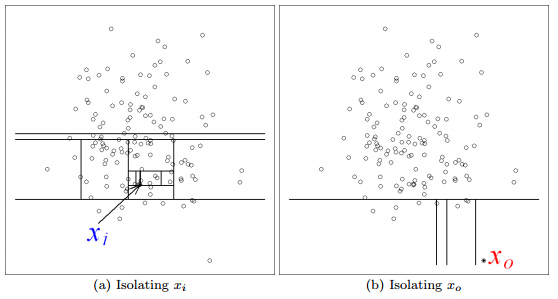
\includegraphics[width=\textwidth]{images/isolation_forest.png}
\caption[Isolation Forest]{Isolation Forest}%
\label{fig:isolation_forest}
\end{figure}
%
Der Anomaly Score wird mit Hilfe der nicht erfolgreichen Suche eines Binary Search Tree berechnet. Dabei ist n die Anzahl Knoten, E(h(x)) die durchschnittliche Pfadlänge und c(n) die durchschnittliche Kostenfunktion einer nicht erfolgreichen Suche im Binary Search Tree. Die Formel dafür sieht wie folgt aus:
\begin{equation}
\label{eq:isolation}
s(x, n) = 2^(-\frac{E(h(x))}{c(n)})
\end{equation}
\newline
Die Funktion s(x, n) gibt immer einen Wert zwischen 0 und 1 zurück. Wobei 1 einem klarem Ausreisser entspricht \cite{isolation_forest_2}.